\chapter{Contexte général du projet}
\begin{onehalfspace}

\initial{L}e présent chapitre permet de situer le projet dans son contexte général, à travers la présentation de l'organisme d'accueil \emph{Sayoo} et des différents services qu'il offre. Nous exposerons aussi les motivations, les objectifs visés ainsi que la planification du projet.

\newpage


\section{Présentation de l'organisme d'accueil}

\textbf{Sayoo} est une Start-up qui agit dans le domaine des technologies de l'information. Lancée en décembre 2013, elle vise à fournir aux clients les solutions adéquates à leurs besoins en utilisant les dernières technologies. \emph{Sayoo} repose principalement sur l’open-source afin de fournir leurs services à prix abordable et bénéficier des communautés actives. 


%\subsection{Organisation}

\subsection{Services}
La société \emph{Sayoo} fournit des services de qualité qui touchent plusieurs domaines.
\paragraph*{Développement logiciel}
\emph{Sayoo} utilise des outils et frameworks performants et récents pour mieux gérer les projets et gagner en terme de coût et temps.

\paragraph*{Développement Web/Mobile}
Le développement mobile tient un place importante au sein de l'entreprise parce que le marché mobile est en constante progression en offres et demandes. 

\paragraph*{Conception des design}
\emph{Sayoo} ne se focalise pas totalement sur l'aspect technique. la société conçoit et délivre des interfaces réactives et séduisantes pour les clients.

\index{Odoo}

\paragraph*{Intégration des \acrshort{erp} et formations}
\emph{Sayoo} se penche aussi sur la gestion des entreprises via Odoo (anciennement Open \acrshort{erp}). Ce service tient une place importante pour la société notamment dans sa personnalisation.

\section{Cadre du projet}


\subsection{Présentation du projet}
 
la Société \emph{Sayoo} tient à fournir des services de qualité à ses clients. Le projet consiste à améliorer le service \emph{\acrshort{erp}} fournit pour les entreprises.

Le service \emph{\acrshort{erp}} tient une importance capitale au sein de la société parce qu'il déploie des ressources importantes. Par ailleurs, toute relation avec une entreprise nécessite une rigueur et une grande attention.

Un client qui désire gérer les ressources de son entreprise  doit rencontrer un responsable de la clientèle de \emph{Sayoo} pour spécifier ses besoins. Le responsable propose une version personnalisée de la suite \emph{Odoo} (anciennement \emph{Open \acrshort{erp}}) au client pour une gestion efficace. Par la suite, la société qui s'est déjà procurée  3 différents serveurs (Développement, Évaluation, Production) doit déployer une version de \emph{Odoo} sur le serveur de développement pour que les développeurs effectuent les premières personnalisations. Le client doit avoir accès au serveur Développement pour confirmer ou refuser. En cas de confirmation, l'administration doit déployer la version souhaitée sur le serveur production et conserver la version d'évaluation au cas d'une nouvelle mise à jour ou maintenance.Le serveur Évaluation a pour but de faire découvrir le client une version standard ou améliorée de la suite \emph{Odoo}.  

Pour une meilleure fiabilité, la société se procure 2 serveurs ( Développement, Production) par client. elle doit périodiquement effectuer des maintenances pour assurer la disponibilité de son service. Chaque client de la société se différencie seulement par sa personnalisation de la suite \emph{Odoo} donc les étapes de configuration sont redondantes pour tous les clients. Le temps de configuration et de déploiement reste important donc le client doit attendre pour accéder à son service après chaque maintenance. Les pré-requis de ce service sont relativement coûteux et affecte par conséquent le prix final du client.
  
















\subsection{Motivations}

Le processus de la provision des applications \acrshort{erp} pour les clients n'est pas optimale. D'où les motivations d'opter vers une solution Cloud. Voici une liste des problèmes que rencontrent \emph{Sayoo} lors du processus du déploiement actuel.

\begin{itemize}

\item La provision des instances \emph{Odoo} est complètement manuelle. Quand un client demande une version de test d'\emph{Odoo} par exemple, l'équipe de \emph{Sayoo} est contrainte d'exécuter une série d'étapes répétitives à partir de la commande, l'installation et la configuration du serveur jusqu'à la mise en place de l'application \emph{Odoo}, configuration DNS, etc...

\item Le besoin récurrent des administrateurs qui doivent garder en permanence l’œil sur les applications des clients.

\item La supervision est manuelle. En effet, au fur et à mesure que le nombre de clients augmente, l'administrateur doit ajouter les applications au système de supervision. Ce processus devient faible et non évolutif. Par conséquent, le suivi est pénible en terme de ressources et temps.

\item L’absence d'automatisme fait que l'équipe \emph{Sayoo} consacre la plupart du temps aux tâches répétitives au lieu de se consacrer au développement et la personnalisation des applications \emph{Odoo}. 

\item La nécessité d'acheter un serveur pour chaque client pour y installer son application, ceci est un "\emph{overkill}" pour atteindre le but. De plus, cela affecte le coût de la solution.

\item L'absence d'une architecture robuste qui peut garantir des exigences non fonctionnelles énormes, à savoir la configuration automatique, la haute disponibilité, la sécurité et la scalabilité. Ainsi, Sayoo ne garantie pas un \acrshort{sla} à ses clients.

\end{itemize}




\section{Objectifs du projet}
Ce projet vise principalement à améliorer le service \emph{\acrshort{erp}} au sein de \emph{Sayoo} par l'automatisation de certaines tâches, notamment la configuration et le déploiement. L'objectif de ce projet est de déployer une architecture qui se caractérise par une haute disponibilité, une scalabilité et une sécurité sans faille. Par conséquent, cela revient à déployer une architecture \emph{Cloud} qui répond aux exigences suivantes.
\begin{itemize}

\item Faciliter la configuration et le déploiement des instances \emph{Odoo} pour les clients.

\item Éviter les tâches répétitives et faciliter la personnalisation de \emph{Odoo}.

\item Réduire le coût en terme de temps et d'argent pour \emph{Sayoo}.

\item Inclure un mécanisme de supervision fiable et évolutif.

\item Gérer aisément plusieurs clients en même temps.  
 
 \end{itemize}






\section{Planification du projet}

Notre projet est loin d'être classique. En effet, il fait appel aux technologies non abordées le long de notre parcours scolaire. Du coup, une planification rigoureuse s'est imposé pour prévoir le déroulement du projet. Grâce aux réunions tenues avec les encadrants au sein de \emph{Sayoo}, nous avons été éclairés sur les différentes étapes du projet ainsi que leurs séquencements. Le projet est partagé en trois grandes étapes : la première est une phase de documentation dont les objectifs est de bien assimiler les nouveaux concepts concernant le Cloud Computing, d'autre part de délimiter le périmètre du projet au niveau fonctionnel qu'au niveau technique. La seconde partie est consacrée à la conception de la solution, quant à la troisième étape, elle traite la mise en œuvre de la solution à travers la réalisation, les tests, et le déploiement.

Le stage a débuté le 23 mars pour une durée de 4 mois. Il en résulte le planning suivant :

\begin{figure}[H]
\centering
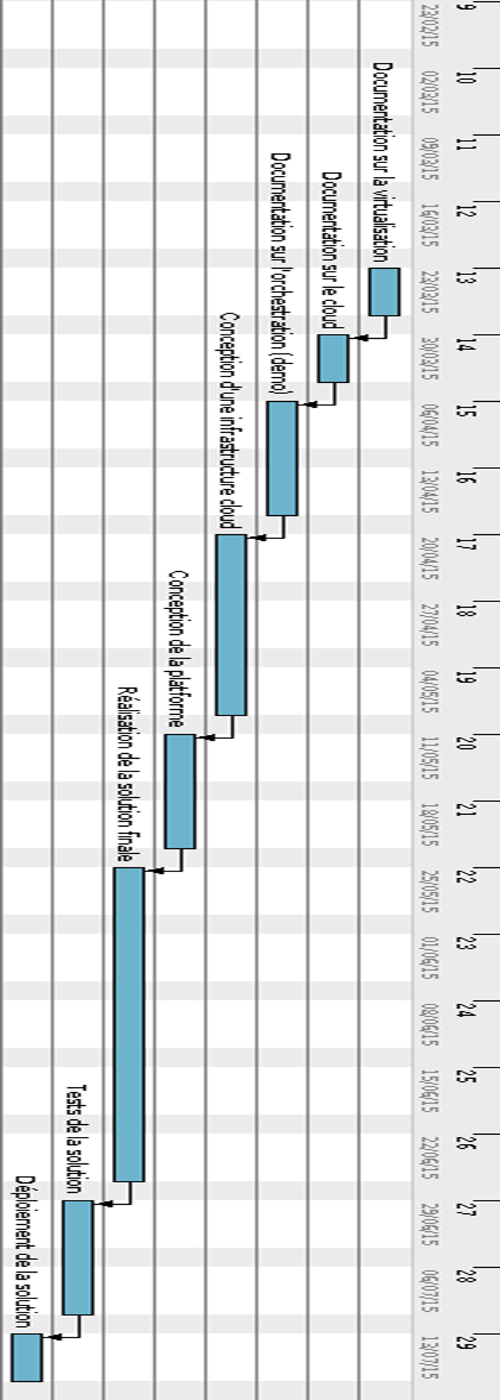
\includegraphics [scale=0.6]{chapitre1/assets/gantt.png}
\caption{Diagramme de Gantt}
\end{figure}


\end{onehalfspace}
